\documentclass[aspectratio=169,compress]{beamer}
  \useoutertheme[footline=authorinstitute,subsection=false]{miniframes}
  \useinnertheme{circles}
  \usefonttheme{default}

  \definecolor{palatinate}{RGB}{126,49,123}
  \definecolor{pale-palatinate}{RGB}{216,172,214}
  \definecolor{grey-palatinate}{RGB}{150,142,133}
  \definecolor{gold-palatinate}{RGB}{159,161,97}
  \definecolor{blue-palatinate}{RGB}{0,99,136}

  \setbeamercolor*{palette primary}{fg=blue-palatinate}
  \setbeamercolor*{palette secondary}{fg=palatinate,bg=pale-palatinate}
  \setbeamercolor*{palette tertiary}{fg=white,bg=palatinate}
  \setbeamercolor*{palette quaternary}{fg=white,bg=gold-palatinate}

  \setbeamercolor*{normal text}{parent=palette primary}
  \setbeamercolor*{footline}{parent=palette secondary}
  \setbeamercolor*{headline}{parent=palette tertiary}
  \setbeamercolor*{titlelike}{parent=palette secondary}

  \setbeamercolor*{structure}{parent=normal text}
  \setbeamercolor*{title in head/foot}{parent=headline}
  \setbeamercolor*{section in head/foot}{parent=headline}
  \setbeamercolor*{author in head/foot}{parent=footline}
  \setbeamercolor*{institute in head/foot}{parent=footline}

  \setbeamercolor*{alerted text}{parent=normal text,fg=palatinate}

  \setbeamercolor*{block title}{fg=white,bg=blue-palatinate}
  \setbeamercolor*{block body}{parent=normal text,bg=pale-palatinate!5}

  \setbeamercolor*{block title example}{fg=white,bg=gold-palatinate}
  \setbeamercolor*{block body example}{parent=normal text,bg=pale-palatinate!5}

  \setbeamertemplate{bibliography item}[text]
  \setbeamertemplate{blocks}[rounded][shadow=true]
  \setbeamertemplate{frametitle}[default][wd=\textwidth]
  \setbeamertemplate{navigation symbols}{}
  \setbeamertemplate{title page}[default][rounded=true,shadow=true]

  \setbeamerfont{block title}{size=\small}

  \BeforeBeginEnvironment{frame}{\citereset}
  \renewcommand{\footnoterule}{}

\usepackage[bibstyle=science,citestyle=numeric-comp]{biblatex}
  \bibliography{references.bib}
\usepackage{calc}
\usepackage[%
  format=hang,
  labelfont={footnotesize,bf},
  textfont={footnotesize,it}
]{caption}
\usepackage{hyperref}
\usepackage[utf8]{inputenc}
\usepackage{multicol}
\usepackage{siunitx}
\usepackage{textcomp}
\usepackage{tikz}
  \usetikzlibrary{calc}
  \usetikzlibrary{external}
    \tikzexternalize[prefix=tikz/]
  \usetikzlibrary{positioning}
  \usetikzlibrary{shapes.geometric}
  \usetikzlibrary{shapes.misc}
  \usetikzlibrary{decorations.pathmorphing}

  \newcommand\tikznum[1]{{\tikzexternaldisable\tikz[baseline=(char.base)]{%
    \node [%
      circle,
      fill=blue-palatinate,
      text=white,
      inner sep=0.5pt,
      font=\scriptsize
    ] (char) {\textnormal{#1}};}}}

  \newcommand\pgfmathsinandcos[3]{%
    \pgfmathsetmacro#1{sin(#3)}%
    \pgfmathsetmacro#2{cos(#3)}%
  }
  \newcommand\LongitudePlane[3][current plane]{%
    \pgfmathsinandcos\sinEl\cosEl{#2} % elevation
    \pgfmathsinandcos\sint\cost{#3} % azimuth
    \tikzset{#1/.style={cm={\cost,\sint*\sinEl,0,\cosEl,(0,0)}}}
  }
  \newcommand\DrawLongitudeArc[2][1]{
    \LongitudePlane{\angEl}{#2}
    \tikzset{current plane/.prefix style={scale=#1}}
     % angle of "visibility"
    % \pgfmathsetmacro\angVis{atan(sin(#2)*cos(\angEl)/sin(\angEl))} %
    \draw[current plane] (90:1) arc (90:270:1);
    % \draw[current plane,dashed] (\angVis:1) arc (\angVis:\angVis+180:1);
    % \draw[current plane,dashed] (\angVis-180:1) arc (\angVis-180:\angVis:1);
  }
  \newcommand\ClipLongitudeArc[2][1]{
    \LongitudePlane{\angEl}{#2}
    \tikzset{current plane/.prefix style={scale=#1}}
    \clip[current plane] (90:1) arc (90:270:1);
  }

  % Common pic definitions
  \tikzset{
    every picture/.append style={
      >=latex,
      line cap=round,
      line join=round,
    },
    endosome/.pic={%
      \filldraw [
        ultra thick,
        draw=palatinate,
        fill=white,
        decorate,
        decoration={random steps,segment length=#1/3,amplitude=#1/6},
        rounded corners=#1/9,
      ] (0,0) circle (#1);
    },
    nanoparticle/.pic={%
      \shadedraw [%
        ultra thick,
        blue-palatinate,
        pic actions,
        ball color=blue-palatinate
      ] (0,0) circle (#1);
    },
    drug/.pic={%
      \shadedraw [
        palatinate,
        pic actions,
        top color=blue-palatinate!80!white,
        bottom color=blue-palatinate!80!black,
      ] (0,#1/2)
        -- (#1/2,#1/2)
        arc (90:-90:#1/2)
        -- (0,-#1/2)
        -- cycle;
      \shadedraw [
        palatinate,
        pic actions,
        top color=palatinate!80!white,
        bottom color=palatinate!80!black,
      ] (0,-#1/2)
        -- (-#1/2,-#1/2)
        arc (270:90:#1/2)
        -- (0,#1/2)
        -- cycle;
    },
    drug grey/.pic={%
      \shadedraw [
        grey-palatinate,
        pic actions,
        top color=grey-palatinate!40!white,
        bottom color=grey-palatinate!40!black,
      ] (0,#1/2)
        -- (#1/2,#1/2)
        arc (90:-90:#1/2)
        -- (0,-#1/2)
        -- cycle;
      \shadedraw [
        grey-palatinate,
        pic actions,
        top color=grey-palatinate!50!white,
        bottom color=grey-palatinate!50!black,
      ] (0,-#1/2)
        -- (-#1/2,-#1/2)
        arc (270:90:#1/2)
        -- (0,#1/2)
        -- cycle;
    },
    drug pos/.pic={%
      \shadedraw [
        palatinate,
        pic actions,
        top color=palatinate!80!white,
        bottom color=palatinate!80!black,
      ] (0,#1/2)
        -- (#1/2,#1/2)
        arc (90:-90:#1/2)
        -- (0,-#1/2)
        -- cycle;
      \shadedraw [
        palatinate,
        pic actions,
        top color=palatinate!80!white,
        bottom color=palatinate!80!black,
      ] (0,-#1/2)
        -- (-#1/2,-#1/2)
        arc (270:90:#1/2)
        -- (0,#1/2)
        -- cycle;
    },
    ligand/.pic={%
      \shade [%
        top color=gold-palatinate!80!white,
        bottom color=gold-palatinate!80!black,
      ] (15:#1/4) 
        -| (#1,-#1/4)
        -| (#1-#1/8,-#1/4*sin{15})
        -| (#1-1.5*#1/8,-#1/4)
        -- (#1-2.5*#1/8,-#1/4)
        |- (-15:#1/4)
        arc (345:15:#1/4)
        -- cycle;
      \shade [shading angle=180,ball color=gold-palatinate,opacity=0.5] (0,0) circle (#1/10);
    },
    receptor/.pic={%
      \shadedraw [%
        thick,
        palatinate,
        top color=black!80!white,
        bottom color=black!80!black,
      ] (240:#1/3) arc (240:-60:#1/3)
        -- (#1/3,-#1)
        -- (-#1/3,-#1)
        -- cycle;
    },
    lipid/.pic={%
      \foreach \y in {{#1/8},{-#1/8}}
        \draw [
          palatinate,
          decorate,
          decoration={snake,segment length=#1/5,amplitude=#1/20},
        ] (0,\y) -- (-#1,\y);
      \shadedraw [blue-palatinate,ball color=blue-palatinate] (0,0) circle (#1/3);
    },
    lipid grey/.pic={%
      \foreach \y in {{#1/8},{-#1/8}}
        \draw [
          grey-palatinate,
          decorate,
          decoration={snake,segment length=#1/5,amplitude=#1/20},
        ] (0,\y) -- (-#1,\y);
      \shadedraw [grey-palatinate,ball color=grey-palatinate] (0,0) circle (#1/3);
    },
    peg/.pic={%
      \draw [
        pic actions,
        decorate,
        decoration={random steps,segment length=#1/10,amplitude=#1/3},
        rounded corners=#1/10,
      ] (0,0) -- (#1,0);
    },
    pH pos/.pic={%
      \shadedraw [
        red,
        top color=red!80!black,
        bottom color=red!80!white,
        pic actions,
      ] (0,-#1/8) rectangle (#1,#1/8);
    },
    pH neg/.pic={%
      \shadedraw [
        black,
        top color=black!80!black,
        bottom color=black!80!white,
        pic actions,
      ] (0,-#1/8) rectangle (#1,#1/8);
    },
    pH poly/.pic={%
      \shadedraw [
        palatinate,
        top color=palatinate!80!black,
        bottom color=palatinate!80!white,
        pic actions,
      ] (0,-#1/8) rectangle (#1,#1/8);
    },
    protein/.pic={
      \shadedraw [%
        thick,
        blue-palatinate,
        pic actions,
        inner color=blue-palatinate!80!white,
        outer color=blue-palatinate!80!black,
        decorate,
        decoration={random steps,segment length=#1/2,amplitude=#1/2},
        rounded corners=#1/10,
      ] (0,0) circle (#1);
    },
    cell/.pic={
      \shadedraw [%
        thick,
        palatinate,
        pic actions,
        inner color=pale-palatinate!80!white,
        outer color=pale-palatinate!80!black,
        decorate,
        decoration={random steps,segment length=#1/2,amplitude=#1/4},
        rounded corners=#1/4,
      ] (0,0) circle (#1);
      \shade [%
        ball color=palatinate,
      ] (0,0) circle (#1/3);
    },
    cancer cell/.pic={
      \shadedraw [%
        thick,
        pic actions,
        palatinate,
        inner color=pale-palatinate!50!white,
        outer color=pale-palatinate!50!black,
        decorate,
        decoration={random steps,segment length=#1/4,amplitude=#1/4},
        rounded corners=#1/8,
      ] (0,0) circle (#1);
      \shade [%
        ball color=palatinate,
      ] (0,0) circle (#1/3);
    },
    endothelial cell/.pic={
      \shadedraw [%
        thick,
        pic actions,
        palatinate,
        inner color=pale-palatinate!80!white,
        outer color=pale-palatinate!80!black,
        rounded corners=#1/4,
      ] (-#1,-#1/2) rectangle (#1,#1/2);
      \shade [%
        ball color=palatinate,
      ] (0,0) circle (#1/3);
    },
  }

\renewcommand*{\footnotefont}{\tiny}
\renewcommand*{\bibfont}{\tiny}
\newcommand*{\autotitle}{\subsecname\hfill\textbf{\small\secname}}

\author{Russell Maguire}
\title{Nanocarriers for targeted drug delivery}
\subtitle{Benefits and challenges of nanotechnology for medicine}
\institute{ENGI4131 Advanced Semiconductor Devices \and Durham University}
\date{\today}
\logo{\Large
\includegraphics[height=1em]{img/Durham.png}}

\begin{document}{}

\frame{\titlepage}

% \section*{Outline}
% \frame{\tableofcontents}

\section{Introduction}

\subsection{Nanocarrier delivery systems}
\begin{frame}[fragile]{\autotitle}
  \begin{columns}
    \column{0.55\textwidth}
      \begin{block}{Structure, types and features}
        \begin{figure}[h]
          \small
          \centering
          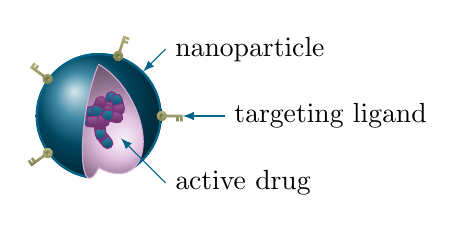
\begin{tikzpicture}
            \def\R{0.8};
            \def\angEl{35};
            \def\angLatA{75};
            \def\angLatB{135};

            \begin{scope}
              \clip (0,0)
                -- ({270-\angEl*cos(\angLatA)}:\R)
                arc ({270-\angEl*cos(\angLatA)}:{-90-\angEl*cos(\angLatB)}:\R)
                -- cycle;
              \pic {nanoparticle=\R};
            \end{scope}
            \foreach \t in {\angLatA,\angLatB} {%
              \pgfmathsetseed{4689}
              \begin{scope}
                \ClipLongitudeArc[\R]{\t};
                \shade [shading angle=180,ball color=pale-palatinate] (0,0) circle (\R);
                \foreach \i in {1,...,15}
                  \pic [rotate=rand*180] at (rand*180:rnd^2*\R/2) {drug=\R/6};
              \end{scope}
              \begin{scope}[line cap=round,draw=pale-palatinate]
                  \DrawLongitudeArc[\R]{\t};
              \end{scope}
            }
            \foreach \t in {72,144,...,216,360}
              \pic [rotate=\t] at (\t:\R) {ligand=\R/3};
            \node [anchor=west,align=left] (nanoparticle) at (45:1.5*\R) {\alert{nanoparticle}};
            \node [anchor=west,align=left] (ligand) at (0:2*\R) {targeting ligand};
            \node [anchor=west,align=left] (drug) at (-45:1.5*\R) {active drug};

            \draw [->,blue-palatinate] (nanoparticle.west) -- (45:\R);
            \draw [->,blue-palatinate] (ligand.west) -- (0:4/3*\R);
            \draw [->,blue-palatinate] (drug.west) -- (-45:\R/2);
          \end{tikzpicture}
          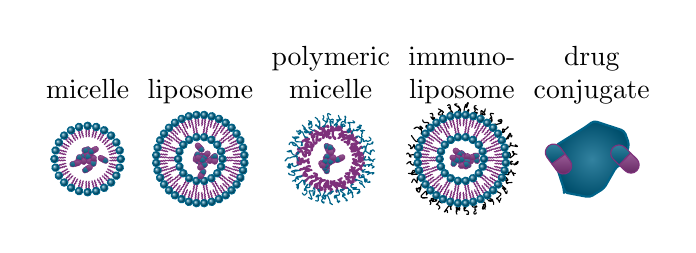
\begin{tikzpicture}
            \def\R{1.2em};
            \pgfmathsetseed{5665};

            \matrix [anchor=base,align=center] {%
              \node {\alert{micelle}}; &
              \node {\alert{liposome}}; &
              \node {\alert{polymeric}\\\alert{micelle}}; &
              \node {\alert{immuno-}\\\alert{liposome}}; &
              \node {\alert{drug}\\\alert{conjugate}}; \\[-1ex]


              % Micelle
              \foreach \t in {15,30,...,360}
                \pic [rotate=\t] at (\t:\R) {lipid=\R/3};
              \foreach \i in {1,...,15}
                \pic [rotate=rand*180,very thin] at (rand*180:rnd^2*\R/2) {drug=\R/6}; &

              % Liposome
              \foreach \t in {20,40,...,360}
                \pic [rotate=180+\t] at (\t:2/3*\R) {lipid=\R/3};
              \foreach \t in {10,20,...,360}
                \pic [rotate=\t+5] at (\t+5:4/3*\R) {lipid=\R/3};
              \foreach \i in {1,...,15}
                \pic [rotate=rand*180,very thin] at (rand*180:rnd^2*\R/2) {drug=\R/6}; &

              % Polymeric micelle
              \foreach \t in {10,20,...,360} {%
                \pic [thick,palatinate,rotate=180+\t] at (\t:\R) {peg=\R/3};
                \pic [blue-palatinate,rotate=\t] at (\t:\R) {peg=\R/3};
              }
              \foreach \i in {1,...,15}
                  \pic [rotate=rand*180,very thin] at (rand*180:rnd^2*\R/2) {drug=\R/6}; &

              % PEGylated liposome
              \foreach \t in {20,40,...,360}
                \pic [rotate=180+\t] at (\t:2/3*\R) {lipid=\R/3};
              \foreach \t in {10,20,...,360} {%
                \pic [rotate=\t+5] at (\t+5:4/3*\R) {peg=\R/3};
                \pic [rotate=\t+5] at (\t+5:4/3*\R) {lipid=\R/3}; 
              }
              \foreach \i in {1,...,15}
                \pic [rotate=rand*180,very thin] at (rand*180:rnd^2*\R/2) {drug=\R/6}; &

              % Protein-drug conjugate
              \pic {protein=\R};
              \foreach \x in {{-\R},\R}
                \pic [rotate=rand*180] at (\x,0) {drug=\R/2}; \\
            };
          \end{tikzpicture}
          \caption{Structure of common types of nanocarriers}
        \end{figure}
      \end{block}

    \column{0.45\textwidth}
      \begin{block}{Definition: nanocarrier}
        \begin{itemize}
          \item Biocompatible nanoparticle encapsulating a drug
        \end{itemize}
      \end{block}

      \begin{block}{Characteristics}
        \begin{columns}[t,onlytextwidth]\small
          \column{0.55\textwidth}\vskip-1em
            \begin{itemize}
              \item \alert{Nanometer scale}
              \item \alert{Biodegradable}
              \item \alert{Non-immunogenic}
              \item \alert{Long half-life}
            \end{itemize}
          \column{0.45\textwidth}\vskip-1em
            \begin{itemize}
              \item \alert{Low toxicity}
              \item \alert{Hydrophilic}
              \item \alert{Soluble}
            \end{itemize}
        \end{columns}
      \end{block}

  \end{columns}
\end{frame}

\subsection{Targeted drug delivery}
\begin{frame}[fragile]{\autotitle}
  \begin{columns}

    \column{0.5\textwidth}
      \begin{block}{How is targeted drug delivery effective?}
        \begin{figure}
          \small
          \centering
          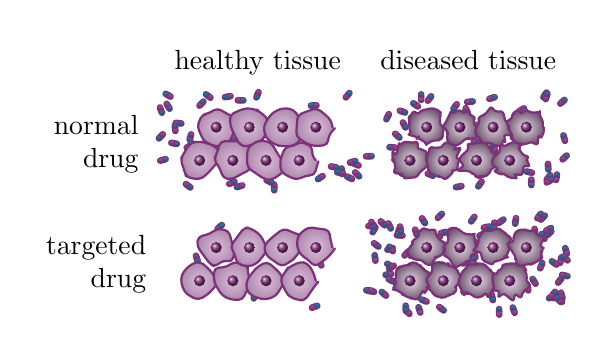
\begin{tikzpicture}
            \def\R{0.6em};
            \pgfmathsetseed{1561};

            \matrix [anchor=center] {%

              &
              \node {\strut\alert{healthy tissue}}; &
              \node {\strut\alert{diseased tissue}}; \\

              \node [align=right] {normal\\drug}; &

              % Normal healthy tissue
              \foreach \i in {1,...,50}
                \pic [rotate=rand*180] at (rand*6*\R,rand*3*\R) {drug=\R/3};
              \foreach \x in {-3,-1,...,3}
                \foreach \y in {-1,1}
                  \pic at ({(\x+\y/2)*\R},\y*\R) {cell=\R}; &

              % Normal diseased tissue
              \foreach \i in {51,...,100}
                \pic [rotate=rand*180] at (rand*6*\R,rand*3*\R) {drug=\R/3};
              \foreach \x in {-3,-1,...,3}
                \foreach \y in {-1,1}
                  \pic at ({(\x+\y/2)*\R},\y*\R) {cancer cell=\R}; \\[\R]

              \node [align=right] {targeted\\drug}; &

              % Untargeted healthy tissue
              \foreach \i in {1,...,5}
                \pic [rotate=rand*180] at (rand*6*\R,rand*3*\R) {drug=\R/3};
              \foreach \x in {-3,-1,...,3}
                \foreach \y in {-1,1}
                  \pic at ({(\x+\y/2)*\R},\y*\R) {cell=\R}; &

              % Targetted diseased tissue
              \foreach \i in {6,...,100}
                \pic [rotate=rand*180] at (rand*6*\R,rand*3*\R) {drug=\R/3};
              \foreach \x in {-3,-1,...,3}
                \foreach \y in {-1,1}
                  \pic at ({(\x+\y/2)*\R},\y*\R) {cancer cell=\R}; \\
            };
          \end{tikzpicture}
          \caption{Goal is to increase drug concentration ratio for diseased tissue}
        \end{figure}
      \end{block}

    \column{0.5\textwidth}
      \begin{block}{Targets diseased tissue}
        \begin{itemize}
          \item Maximise therapeutic effects
          \item Minimise effective drug dose
          \item Common targets are \alert{solid~tumours}, \alert{inflamed} and \alert{infected~tissue}
        \end{itemize}
      \end{block}

      \begin{block}{Avoids healthy tissue}
        \begin{itemize}
          \item Minimise toxic side-effects
        \end{itemize}
      \end{block}

  \end{columns}
\end{frame}

\section{Passive targeting}

\subsection{Enhanced permeability and retention effect}
\begin{frame}[fragile]{\autotitle}
  \begin{columns}
    \column{0.5\textwidth}
      \begin{beamercolorbox}[rounded=true,shadow=true]{titlelike}\small
          Basis for \textbf{first generation} nanomedicines~\footcitemark{wicki2015nanomedicine}
      \end{beamercolorbox}

      \begin{block}{Illustration of the EPR effect}
        \begin{figure}
          \small
          \centering
          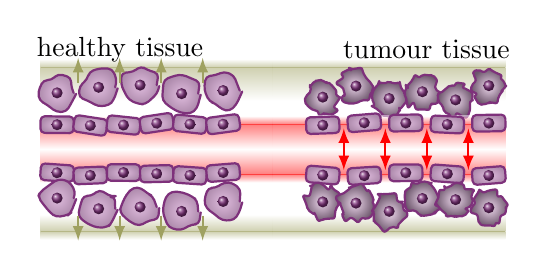
\begin{tikzpicture}
            \def\R{0.6em};
            \def\wallsep{4*\R};
            \pgfmathsetseed{9425};

            \matrix (m) [anchor=center] {%

              % Upper healthy tissue
              \shade [
                top color=gold-palatinate!0,
                bottom color=gold-palatinate,
                opacity=0.5,
              ] (-6*\R,1.5*\R) rectangle (6*\R+\wallsep/2,2*\R);
              \shade [
                top color=gold-palatinate,
                bottom color=gold-palatinate!0,
                opacity=0.5,
              ] (-6*\R,1.5*\R) rectangle (6*\R+\wallsep/2,-0.5*\R);
              \foreach \x in {-4,-2,...,4}
                \pic at (5/4*\x*\R,rand*\R/2) {cell=\R}; &

              % Upper tumour tissue
              \shade [
                top color=gold-palatinate!0,
                bottom color=gold-palatinate,
                opacity=0.5,
              ] (-6*\R-\wallsep/2,1.5*\R) rectangle (6*\R,2*\R);
              \shade [
                top color=gold-palatinate,
                bottom color=gold-palatinate!0,
                opacity=0.5,
              ] (-6*\R-\wallsep/2,1.5*\R) rectangle (6*\R,-0.5*\R);
              \foreach \x in {-5,-3,...,5}
                \pic at (\x*\R,rand*\R/2) {cancer cell=\R}; \\[-\R/2]
              
              % Upper healthy capillary wall
              \shade [
                top color=red!0,
                bottom color=red,
                opacity=0.5,
              ] (-6*\R,0) rectangle (6*\R+\wallsep/2,0.5*\R);
              \shade [
                top color=red,
                bottom color=red!0,
                opacity=0.5,
              ] (-6*\R,0) rectangle (6*\R+\wallsep/2,-1.5*\R);
              \foreach \x in {-5,-3,...,5}
                \pic [rotate=rand*10] at (\x*\R,rand*\R/8) {endothelial cell=\R}; &

              % Upper tumour capillary wall
              \shade [
                top color=red!0,
                bottom color=red,
                opacity=0.5,
              ] (-6*\R-\wallsep/2,0) rectangle (6*\R,0.5*\R);
              \shade [
                top color=red,
                bottom color=red!0,
                opacity=0.5,
              ] (-6*\R-\wallsep/2,0) rectangle (6*\R,-1.5*\R);
              \foreach \x in {-4,-2,...,4}
                \pic [rotate=rand*5] at (5/4*\x*\R,rand*\R/8) {endothelial cell=\R}; \\

              % Lower healthy capillary wall 
              \shade [
                top color=red!0,
                bottom color=red,
                opacity=0.5,
              ] (-6*\R,0) rectangle (6*\R+\wallsep/2,1.5*\R);
              \shade [
                top color=red,
                bottom color=red!0,
                opacity=0.5,
              ] (-6*\R,0) rectangle (6*\R+\wallsep/2,-0.5*\R);
              \foreach \x in {-5,-3,...,5}
                \pic [rotate=rand*5] at (\x*\R,rand*\R/8) {endothelial cell=\R}; &

              % Lower tumour capillary wall
              \shade [
                top color=red!0,
                bottom color=red,
                opacity=0.5,
              ] (-6*\R-\wallsep/2,0) rectangle (6*\R,1.5*\R);
              \shade [
                top color=red,
                bottom color=red!0,
                opacity=0.5,
              ] (-6*\R-\wallsep/2,0) rectangle (6*\R,-0.5*\R);
              \foreach \x in {-4,-2,...,4}
                \pic [rotate=rand*5] at (5/4*\x*\R,rand*\R/8) {endothelial cell=\R}; \\[-\R/2]

              % Lower healthy tissue
              \shade [
                top color=gold-palatinate!0,
                bottom color=gold-palatinate,
                opacity=0.5,
              ] (-6*\R,-1.5*\R) rectangle (6*\R+\wallsep/2,-0.5*\R);
              \shade [
                top color=gold-palatinate,
                bottom color=gold-palatinate!0,
                opacity=0.5,
              ] (-6*\R,-1.5*\R) rectangle (6*\R+\wallsep/2,-2*\R);
              \foreach \x in {-4,-2,...,4} 
                \pic at (5/4*\x*\R,rand*\R/2) {cell=\R}; &

              % Lower tumour tissue
              \shade [
                top color=gold-palatinate!0,
                bottom color=gold-palatinate,
                opacity=0.5,
              ] (-6*\R-\wallsep/2,-1.5*\R) rectangle (6*\R,-0.5*\R);
              \shade [
                top color=gold-palatinate,
                bottom color=gold-palatinate!0,
                opacity=0.5,
              ] (-6*\R-\wallsep/2,-1.5*\R) rectangle (6*\R,-2*\R);
              \foreach \x in {-5,-3,...,5} 
                \pic at (\x*\R,rand*\R/2) {cancer cell=\R}; \\
            };

            \foreach \x in {-3,-1,...,3}
              \foreach \y in {-1,1} {
                \begin{scope}[%
                  ->,
                  line cap=butt,
                  thick,
                ]
                  \pgfmathsetmacro{\X}{(6+5/4*\x)};
                  \draw [red] (\X*\R+\wallsep/2,0) -- (\X*\R+\wallsep/2,1.25*\y*\R);
                  \draw [gold-palatinate] (-\X*\R-\wallsep/2,4*\y*\R) -- (-\X*\R-\wallsep/2,5.5*\y*\R);
                \end{scope}
              };
            \node [anchor=base,right=0 of m.north west] {\alert{healthy tissue}};
            \node [anchor=base,left=0 of m.north east] {\alert{tumour tissue}};
          \end{tikzpicture}
          \caption{\textcolor{gold-palatinate}{Lymphatic system} drainage and \textcolor{red!80}{blood vessel} permeability in solid tumours}
        \end{figure}
      \end{block}

    \column{0.5\textwidth}
      \begin{block}{Definition: EPR effect}
        \begin{itemize}
          \item Tendency for nanoparticles to accumulate in \alert{solid~tumours}~\footcitemark{maeda2000tumor}
        \end{itemize}
      \end{block}

      \begin{block}{Accumulation procedure}
        \begin{enumerate}
          \item Molecules leak from blood into tissue due to \alert{enhanced vascular permeability}
          \item \alert{Blocked lymphatic system} due to dense rapidly growing tumour cells~\footcitemark{padera2004pathology}
          \item Large particles become trapped
        \end{enumerate}
      \end{block}

  \end{columns}\vskip-0.2em
  \footcitetext{maeda2000tumor,wicki2015nanomedicine,padera2004pathology}
\end{frame}

\section{Stimuli-responsive targeting}

\subsection{Internal stimuli-responsive nanocarriers}
\begin{frame}[fragile]{\autotitle}
  \begin{columns}
    \column{0.5\textwidth}
      \begin{example}
        \begin{figure}[h]
          \small
          \centering
          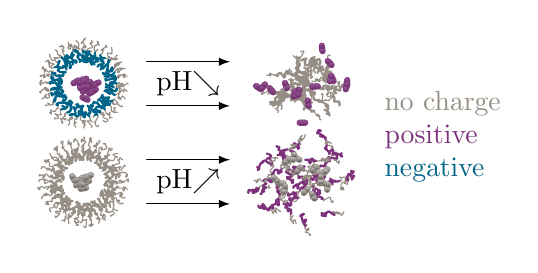
\begin{tikzpicture}
            \def\R{1.2em};
            \def\arrowlen{4*\R};
            \pgfmathsetseed{7756};

            \matrix (m) [column sep=\R/2] {%

              % Charged micelle
              \foreach \t in {10,20,...,360} {
                \pic [grey-palatinate,rotate=\t] at (\t:\R) {peg=\R/3};
                \pic [thick,blue-palatinate,rotate=180+\t] at (\t:\R) {peg=\R/3};
              };
              \foreach \i in {1,...,15}
                  \pic [rotate=rand*180,very thin] at (rand*180:rnd^2*\R/2) {drug pos=\R/6}; &

              \node (pH) {pH$\searrow$};
              \draw [->] (pH.north west) -- (pH.north east);
              \draw [->] (pH.south west) -- (pH.south east); &

              % Collapsed charged micelle
              \foreach \t in {10,20,...,360} {
                \pgfmathsetmacro{\randA}{rand}
                \pgfmathsetmacro{\randB}{rand}
                \pgfmathsetmacro{\rnd}{rnd}
                \pic [grey-palatinate,rotate=\randA*180] at (\randB*180:\rnd*\R) {peg=\R/3};
                \pic [thick,grey-palatinate,rotate=180+\randA*180] at (\randB*180:\rnd*\R) {peg=\R/3};
              };
              \foreach \i in {1,...,15}
                  \pic [rotate=rand*180,very thin] at (rand*180:rnd*1.5*\R) {drug pos=\R/6}; \\

              % Neutral micelle
              \foreach \t in {10,20,...,360} {
                \pic [grey-palatinate,rotate=\t] at (\t:\R) {peg=\R/3};
                \pic [thick,grey-palatinate,rotate=180+\t] at (\t:\R) {peg=\R/3};
              };
              \foreach \i in {1,...,15}
                  \pic [rotate=rand*180,very thin] at (rand*180:rnd^2*\R/2) {drug grey=\R/6}; &

              \node (pH) {pH$\nearrow$};
              \draw [->] (pH.north west) -- (pH.north east);
              \draw [->] (pH.south west) -- (pH.south east); &

              % Collapsed neutral micelle
              \foreach \t in {10,20,...,360} {
                \pgfmathsetmacro{\randA}{rand}
                \pgfmathsetmacro{\randB}{rand}
                \pgfmathsetmacro{\rnd}{rnd}
                \pic [grey-palatinate,rotate=\randA*180] at (\randB*180:\rnd*1.5*\R) {peg=\R/3};
                \pic [thick,palatinate,rotate=180+\randA*180] at (\randB*180:\rnd*1.5*\R) {peg=\R/3};
              };
              \foreach \i in {1,...,15}
                  \pic [rotate=rand*180,very thin] at (rand*180:rnd*\R) {drug grey=\R/6}; \\
            };

            \node [align=left,right=0 of m.east] {
              \textcolor{grey-palatinate}{$\blacksquare$ no charge} \\
              \textcolor{palatinate}{$\blacksquare$ positive} \\
              \textcolor{blue-palatinate}{$\blacksquare$ negative}
            };
          \end{tikzpicture}
          \caption{Polymeric micelles with pH-responsive polymers for electrostatic release~\footcitemark{sun2014engineered}}
        \end{figure}
      \end{example} 

    \column{0.5\textwidth}
      \begin{block}{Bioindicators used to trigger release}
        \begin{columns}[t,onlytextwidth]
          \column{0.5\textwidth}\vskip-1em
            \begin{itemize}
              \item \alert{pH level}
              \item \alert{Enzymes}
            \end{itemize}
          \column{0.5\textwidth}\vskip-1em
            \begin{itemize}
              \item \alert{Redox potential}
              \item \alert{Temperature}
            \end{itemize}
        \end{columns}
      \end{block}

      \begin{block}{Target sites for pH-responsive nanocarriers}
        \begin{itemize}
          \item \alert{Tumours} have been observed with lower pH than healthy tissue~\footcitemark{tannock1989acid,gerweck1996cellular}
          \item Individual \alert{organelles} within the cell maintain their own unique pH~\footcitemark{wicki2015nanomedicine}
        \end{itemize}
      \end{block}

  \end{columns}
  \footcitetext{sun2014engineered,gerweck1996cellular,tannock1989acid,wicki2015nanomedicine}
\end{frame}

\subsection{External stimuli-responsive nanocarriers}
\begin{frame}[fragile]{\autotitle}
  \begin{columns}
    \column{0.5\textwidth}
      \begin{example}
        \begin{figure}[h]
          \small
          \centering
          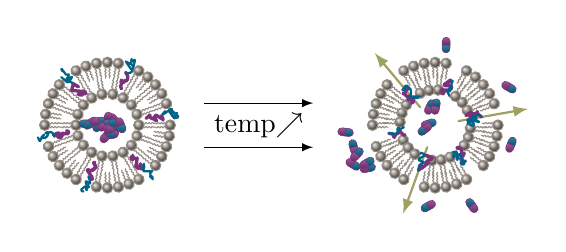
\begin{tikzpicture}
            \def\R{1.7em};
            \pgfmathsetseed{4456}

            \matrix [column sep=\R/2] {

              % Themosensitive liposome
              \foreach \t in {20,40,...,360}
                \pic [rotate=180+\t] at (\t:2/3*\R) {lipid grey=\R/3};
              \foreach \t in {60,120,...,360} {%
                \foreach \h in {10,20,...,50}
                  \pic [rotate=\t+\h+10] at (\t+\h+10:4/3*\R) {lipid grey=\R/3};
                \pic [rotate=180+\t+10,very thick,palatinate] at (\t+10:7/6*\R) {peg=\R/3};
                \pic [rotate=\t+10,thick,blue-palatinate] at (\t+10:7/6*\R) {peg=\R/3};
              };
              \foreach \i in {1,...,15}
                \pic [rotate=rand*180,very thin] at (rand*180:rnd^2*\R/2) {drug=\R/6}; &

              \node (T) {temp$\nearrow$};
              \draw [->] (T.north west) -- (T.north east);
              \draw [->] (T.south west) -- (T.south east); &

              % Permeable themosensitive liposome
              \foreach \t in {120,240,360}
                \draw [->,thick,gold-palatinate] (\t+10:\R/2) -- (\t+10:2*\R);
              \foreach \t in {60,120,...,360} {%
                \foreach \h in {15,30,45}
                  \pic [rotate=180+\t+\h+10] at (\t+\h+10:3/4*\R) {lipid grey=\R/3};
                \foreach \h in {10,20,...,50}
                  \pic [rotate=\t+\h+10] at (\t+\h+10:4/3*\R) {lipid grey=\R/3};
                \pic [rotate=165+\t+10,very thick,palatinate] at (\t+10:\R) {peg=\R/3};
                \pic [rotate=195+\t+10,thick,blue-palatinate] at (\t+10:\R) {peg=\R/3};
              };
              \foreach \i in {1,...,4}
                \pic [rotate=rand*180,very thin] at (rand*180:rnd*\R/2) {drug=\R/6};
              \foreach \i in {5,...,15}
                \pic [rotate=rand*180,very thin] at (rand*180:rnd*\R/2+1.5*\R) {drug=\R/6}; \\
            };
          \end{tikzpicture}
          \caption{Liposomes modified with thermosensitive polymers for controlled release~\footcitemark{ta2013thermosensitive,kono2001thermosensitive}}
        \end{figure}
      \end{example}

    \column{0.5\textwidth}
      \begin{block}{Mechanisms used to externally trigger release}
        \begin{columns}[t,onlytextwidth]
          \column{0.65\textwidth}\vskip-1em
            \begin{itemize}
              \item \alert{Electromagnetic fields}
              \item \alert{Ultrasound}
            \end{itemize}
          \column{0.35\textwidth}\vskip-1em
            \begin{itemize}
              \item \alert{Heat}
              \item \alert{Light}
            \end{itemize}
        \end{columns}
      \end{block}

      \begin{block}{Induced local hyperthermia}
        \begin{itemize}
          \item Target temperature is \num{40}--\SI{45}{\degreeCelsius}~\footcitemark{jhaveri2014stimuli,ganta2008review}
          \item Direct heat can be applied to target
          \item Magnetic fields can be used to heat iron oxide nanoparticles at target~\footcitemark{scherer2002magnetofection}
        \end{itemize}
      \end{block}

  \end{columns}\vskip-0.4em
  \footcitetext{ta2013thermosensitive,jhaveri2014stimuli,scherer2002magnetofection,ganta2008review,kono2001thermosensitive}
\end{frame}

\section{Active targeting}

\subsection{Nanocarriers with surface ligands}
\begin{frame}[fragile]{\autotitle}
  \begin{columns}
    \column{0.5\textwidth}
      \begin{block}{Receptor-mediated endocytosis of nanocarriers}
        \begin{figure}[h]
          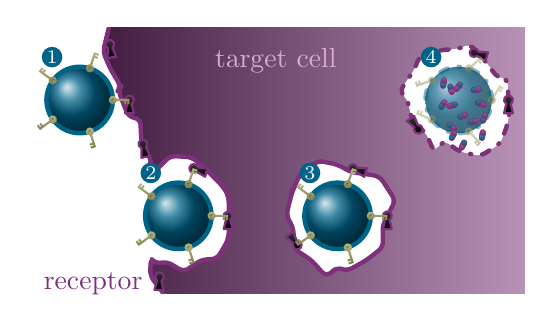
\begin{tikzpicture}
            \def\R{1.2em};
            \pgfmathsetseed{9845};

            % Cell wall
            \begin{scope}
              \clip (-6*\R,-4*\R) rectangle (7.5*\R,4*\R);
              \shadedraw [%
                ultra thick,
                palatinate,
                left color=palatinate!50!black,
                right color=palatinate!50!white,
                decorate,
                decoration={random steps,segment length=\R/2,amplitude=\R/4},
                rounded corners=\R/6,
              ] (8*\R,5*\R)
                -- (-5.5*\R,5*\R)
                -- (-3.75*\R,-0.35*\R)
                arc (120:-120:1.5*\R)
                -- (-3*\R,-5*\R)
                -- (8*\R,-5*\R)
                -- cycle;
              \node [text=pale-palatinate] at (0,3*\R) {target cell};

              % Cell wall receptors
              \pic [rotate=rand*15] at (-5*\R,3.5*\R) {receptor=0.4*\R};
              \pic [rotate=rand*15] at (-4*\R,0.5*\R) {receptor=0.4*\R};
              \pic [rotate=rand*15] at (-3.5*\R,-3.5*\R) {receptor=0.4*\R};
            \end{scope}
            \node [text=palatinate] at (-5.5*\R,-3.7*\R) {receptor};

            \matrix [
              nodes={%
                circle,
                anchor=south west,
                fill=blue-palatinate,
                text=white,
                inner sep=0.5pt,
                font=\scriptsize,
              },
            ] {%

              % Step 1: Binding
              \pic at (0:1.5*\R) {receptor=0.4*\R};
              \pic {nanoparticle=\R};
              \foreach \t in {72,144,...,360}
                \pic [rotate=\t] at (\t:\R) {ligand=0.5*\R};
              \node at (135:1.5*\R) {1}; &&[1.5*\R]&

              % Step 4: Drug release
              \pic [loosely dash dot] {endosome=1.5*\R};
              \foreach \t in {72,216,360}
                \pic [rotate=\t] at (\t:1.5*\R) {receptor=0.4*\R};
              \pic [loosely dash dot,opacity=0.5] {nanoparticle=\R};
              \foreach \t in {72,144,...,360}
                \pic [rotate=\t+rand*60,opacity=0.5] at (\t:\R) {ligand=0.5*\R};
              \foreach \i in {1,...,15}
                  \pic [rotate=rand*180,very thin] at (rand*180:rnd*1.5*\R) {drug=\R/6}; 
              \node at (135:1.5*\R) {4}; \\&

              % Step 3: Endocytosis
              \foreach \t in {72,360}
                \pic [rotate=\t] at (\t:1.5*\R) {receptor=0.4*\R};
              \pic {nanoparticle=\R};
              \foreach \t in {72,144,...,360}
                \pic [rotate=\t] at (\t:\R) {ligand=0.5*\R};
              \node at (135:1.5*\R) {2}; &[1.5*\R]

              % Step 3: Endosome transport
              \pic {endosome=1.5*\R};
              \foreach \t in {72,216,360}
                \pic [rotate=\t] at (\t:1.5*\R) {receptor=0.4*\R};
              \pic {nanoparticle=\R};
              \foreach \t in {72,144,...,360}
                \pic [rotate=\t] at (\t:\R) {ligand=0.5*\R}; 
              \node at (135:1.5*\R) {3}; \\
            };
          \end{tikzpicture}
          \caption{Nanocarrier binding~\tikznum{1}, endocytosis~\tikznum{2}, endosome transport~\tikznum{3}, and drug release~\tikznum{4}}
        \end{figure}
      \end{block}

    \column{0.5\textwidth}
      \begin{block}{Definition: active targeting}
        \begin{itemize}
            \item Targeted drug delivery to specific cell types by encouraging cell uptake
        \end{itemize}
      \end{block}

      \begin{block}{Cell uptake procedure}
        \begin{enumerate}
            \item Passive targeting delivers nanocarrier to solid tumour, \emph{eg.} via EPR effect~\footcitemark{maeda2000tumor}
            \item Surface \alert{ligands} on nanocarrier bind to surface \alert{receptors} on target cell
            \item Cell absorbs nanocarrier via \alert{receptor-mediated endocytosis}~\footcitemark{sun2014engineered}
        \end{enumerate}
      \end{block}

  \end{columns}
  \footcitetext{maeda2000tumor,sun2014engineered}
\end{frame}


\section{Examples}

\subsection{Nanocarrier chemotherapy drugs on the market}
\begin{frame}{\autotitle}
  \begin{columns}
    \column{0.5\textwidth}
      \begin{block}{Doxil\textsuperscript{\textregistered}/Caelyx\textsuperscript{\textregistered}~\footcitemark{harrison1995liposomal}}
        \begin{itemize}
          \item \alert{\emph{Peg}ylated liposomal \emph{doxorubicin}}
          \item \alert{Immunoliposome} using \emph{polyethylene glycol} (\emph{PEG}) stealth coating
          \item \alert{Passively targeted} \emph{doxorubicin}
          \item Reduced cardiac side effects~\footcitemark{wicki2015nanomedicine}
          \item Clinical trials are exploring \alert{actively targeted variations}~\footcitemark{mamot2012tolerability}
        \end{itemize}
      \end{block}

    \column{0.5\textwidth}
      \begin{block}{Abraxane\textsuperscript{\textregistered}~\footcitemark{desai2006increased}}
        \begin{itemize}
          \item \alert{Nanoparticle \emph{albumin}-bound \emph{paclitaxel}}
          \item \alert{Protein-drug conjugate}---\emph{albumin} is a common transport protein in blood
          \item \alert{Passively targeted} \emph{paclitaxel}
          \item Improved solubility~\footcitemark{wicki2015nanomedicine}
          \item Unavailable on NHS from 2015--2017, partly due to cost~\footcitemark{nice2015paclitaxel}
        \end{itemize}
      \end{block}

  \end{columns}
  \footcitetext{wicki2015nanomedicine,harrison1995liposomal,mamot2012tolerability,desai2006increased,nice2015paclitaxel}
\end{frame}

\begin{frame}
  \begin{beamercolorbox}[rounded=true,shadow=true,sep=8pt]{titlelike}\centering\Large
    Thank you, any questions?
  \end{beamercolorbox}
  \begin{block}{References}\bibfont
    \begin{multicols}{2}[\vskip-1em]
      \printbibliography
    \end{multicols}
  \end{block}
\end{frame}

\end{document}
